\documentclass[11pt]{beamer}
\usetheme{Warsaw}
\usepackage[T1]{fontenc}
%\usepackage[utf8]{inputenc}
\usepackage{amsmath}
\usepackage{amsfonts}
\usepackage{amssymb}
\usepackage{graphicx}
\graphicspath{{imgs/}}
\usepackage{setspace}
\usepackage{hyperref}
\usepackage{listings}
\usepackage{xcolor}
%\usepackage{minted}


\author{Chen Zhang \inst{1,2}}
\title{Scientific computation and anomaly recognition}
\setbeamertemplate{enumerate items}[default]


\logo{
\includegraphics[width=.25\textwidth]{UIH-logo.jpg}}

\institute[UNI]{\inst{1}RTL CRI\_SZ UIH $@$ Shenzhen, \inst{2}PMJL RUJC-CRI UIH $@$ Shanghai\\[2.5ex] {Git URL: \href{https://github.com/CubicZebra/}{\color{cyan}\underline{CubicZebra}}}}

\date{}

% customized
\newcommand{\code}[1]{\texttt{#1}}
\newcommand{\asred}[1]{{\color{red}#1}}
\newcommand{\uniitem}[1]{\begin{itemize}\item #1 \end{itemize}}
\newcommand{\ftref}[2]{{\color{blue}\footnotesize \href{#1}{#2}}}
\AtEndDocument{\begin{frame}{\huge \quad Thanks.}\end{frame}}

\definecolor{comment}{rgb}{0, 0.6, 0}
\definecolor{keyword}{rgb}{0.96, 0.52, 0.02}
\definecolor{string}{rgb}{0.12, 0.4, 0.87}
\definecolor{background}{rgb}{0.95,0.95,0.92}
\lstdefinestyle{mypython}{
	language=Python,
    backgroundcolor=\color{background},   
    commentstyle=\color{comment},
    keywordstyle=\color{keyword},
    numberstyle=\tiny\color{magenta},
    stringstyle=\color{string},
    basicstyle=\ttfamily\footnotesize,
    breakatwhitespace=false,         
    breaklines=true,                 
    captionpos=b,
    keepspaces=true,
    numbers=left,
    numbersep=5pt,
	showspaces=false,
	showstringspaces=false,
    showtabs=false,
    tabsize=2
}
\lstset{style=mypython}


\begin{document}
\font\nullfont=cmr10  % warn of no nullfont

\begin{frame}
\titlepage
\end{frame}

\begin{frame}
\tableofcontents
\end{frame}

\section{Scientific computation}

\subsection{Motivation: full support of algorithm}

\begin{frame}{Essence: utilizing the valuable pattern from data}
	\begin{itemize}
		\item Program in CS: \\
			\qquad data (digital) + algorithms (business)
		\item Data mining: (purification, \asred{critical}) \\
			\qquad data (conceptual) + algorithms (simplication)
		\item AI application: (utilization) \\
			\qquad data (representation) + algorithms (criterion)
	\end{itemize}
\end{frame}

\begin{frame}{Data mining}
	\uniitem{Pattern: minimal representation of data\footnote[frame]{\ftref{https://informatics.readthedocs.io/en/latest/supplement/supp\_a1.html\#id4}{Pattern in high dimensional data}}}
	\centering
	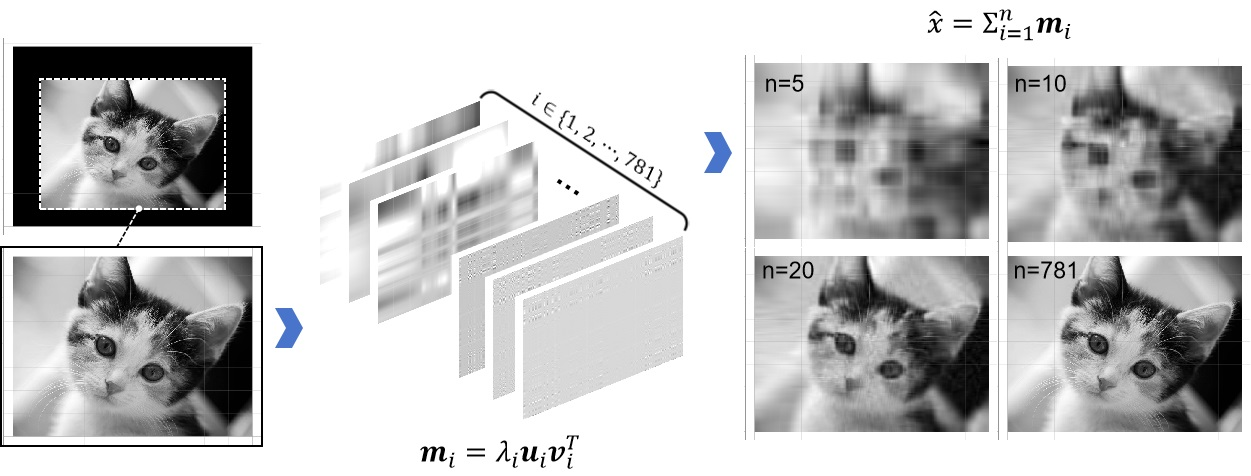
\includegraphics[scale=0.65]{minimal-rep.jpg}
\end{frame}

\begin{frame}{AI application}
	\begin{itemize}
		\item Mathematical statistics: \\
			\qquad hypotest, ANOVA, Bayesian stats, statistical learning, \dots
		\item Machine learning: \\
			\begin{itemize}
				\item analytical: PCA, SVM, conjugate gradient descent, \dots
				\item randomness: RF, ensemble, stochastic gradient descent, \dots
			\end{itemize}
		\item Deep learning: \\
			\begin{itemize}
				\item Conv+Pool (+randomness \& variation, data aug \& mining)
				\item MLP ($p = f(\boldsymbol{x}) \rightarrow f$, set criterion of regressor)
			\end{itemize}
	\end{itemize}
\end{frame}

\begin{frame}{Scientific computation: base implementation of algorithms}
	\uniitem{Signal decomposition
		\uniitem{eigen and sigular value decomp.,}
		\uniitem{tensor decomp. \& synthesis (CP, tucker, train, ring);}}
	\uniitem{Optimization
		\uniitem{linear or nonlinear OLS,}
		\uniitem{gradient descent: (quasi-)newton iter, conjugate, stochastic,}
		\uniitem{stochastic process;}}
	\uniitem{Statistics
		\uniitem{inference: MLE, Bayes (posteriori \& prediction dis), }
		\uniitem{measurement: univariate/multivariate hypothesis tests,}
		\uniitem{sampling: MH, MCMC, stat simulation;}}
	\uniitem{Linear algebra, ODR, PDE, \dots}
\end{frame}

\subsection{Significance: unveil the black box of AI}

\begin{frame}{For rational AI approaches}
	\uniitem{Comprehension on algorithm frame
		\uniitem{What: base components of scientific computation methods,}
		\uniitem{Why: reason of frame architecture design,}
		\uniitem{How: concrete computation steps of each component;}}
	\uniitem{Modification on algorithm frame
		\uniitem{Parameter: inherent adaption support of frame,}
		\uniitem{Component: change features of frame for certain purpose;}}
	\uniitem{Creating customized frame
		\uniitem{Analysis: data \asred{\textbf{=>}} concerned info => sc methods,}
		\uniitem{Architect: sc implements \asred{\textbf{=>}} atomic ops => pipe;}}
\end{frame}

\begin{frame}{For rational AI approaches}
	Two suggestions in practice:
	\begin{enumerate}
		\item \textbf{Deep into principles:} despite autonomous vehicles, a driver inside should have license at least.
		\item \textbf{Don't against the current:} modification/design based on \emph{concerned info} and \emph{task objective}.
	\end{enumerate}
\end{frame}

\begin{frame}{The objective-oriented methodology}
	\uniitem{Case 1: fingerprint recognition\footnote[frame]{\ftref{https://informatics.readthedocs.io/en/latest/tutorial/tut\_aug.html\#gabor-fingerprint-augmentation}{Determine appropriate transformation}}
		\uniitem{interested info: pattern of texture}
		\uniitem{sc methods: spatial gabor filtering (2D)}}
	\centering
	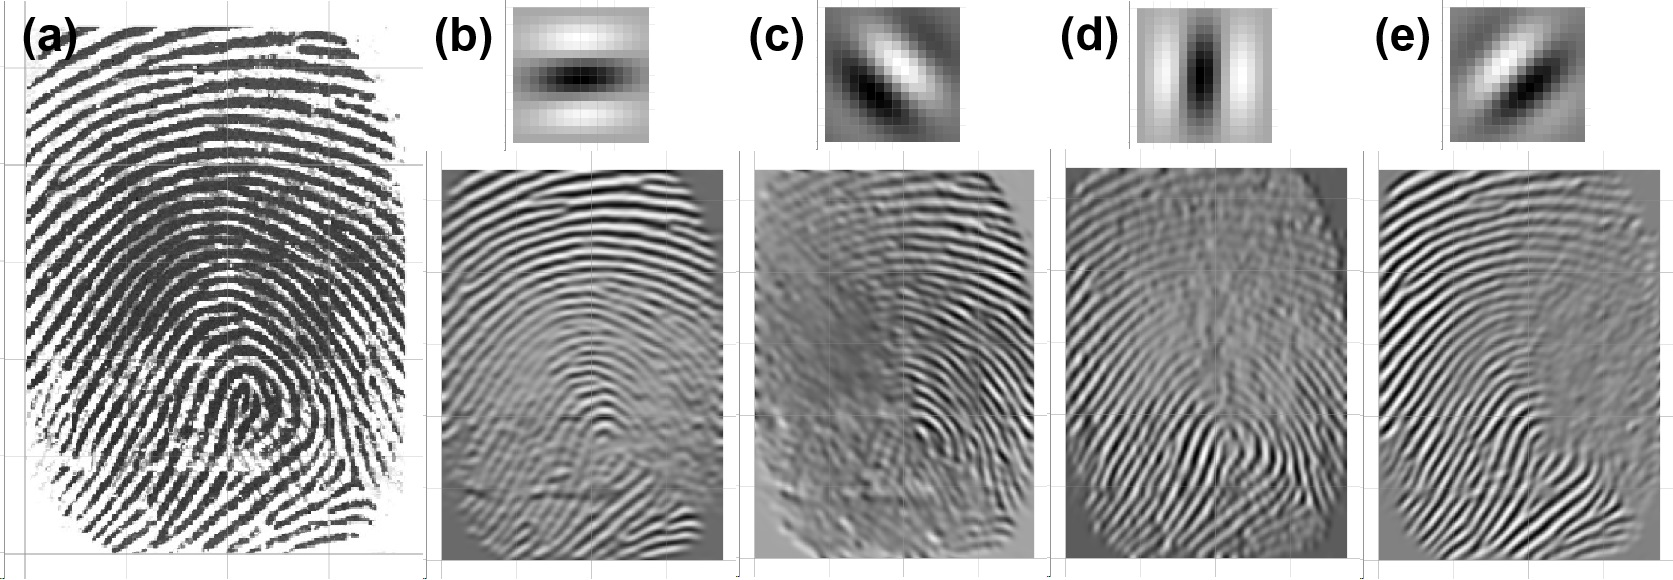
\includegraphics[scale=0.45]{fingerprint.jpg}
\end{frame}

\begin{frame}{The objective-oriented methodology}
	\uniitem{Case 2: vessel measurement in pancreatic carcinoma study
		\uniitem{interested info: space angle}
		\uniitem{sc methods: morphological ops + linalg computation}}
	\centering
	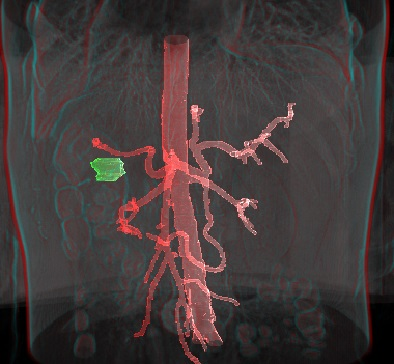
\includegraphics[scale=0.75]{angle.jpg}
\end{frame}

\begin{frame}{The objective-oriented methodology}
	\uniitem{Case 3: brain-related study (pipe reusability in Case 1)
		\uniitem{interested info: texture pattern of brain}
		\uniitem{sc methods: spatial gabor filtering (3D)}}
	\centering
	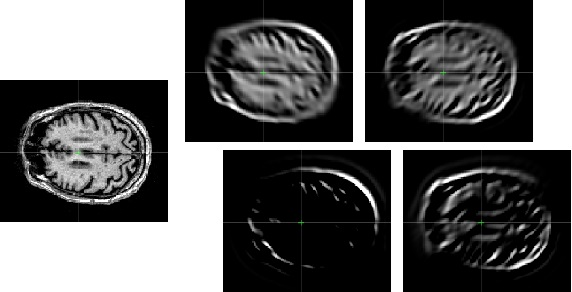
\includegraphics[scale=0.9]{brain.jpg}
\end{frame}

\subsection{Supremum: reduce nonsense efforts}

\begin{frame}{Primer concepts in statistics}
	\uniitem{Why we need statistics
		\uniitem{data: listing all acquired observations}
		\uniitem{statistics: description on data via sth. (e.g. dis)}}
	\uniitem{Samples \& population
		\uniitem{estimation: study on samples => conclusion on population}
		\uniitem{bias: diff between samples \& population\footnote[frame]{\ftref{https://informatics.readthedocs.io/en/latest/supplement/supp\_b2.html\#unbias-estimation}{Unbias estimation}}}}
\end{frame}

\begin{frame}{Primer concepts in statistics}
	\uniitem{Parametric or non-parametric\footnote[frame]{\ftref{https://informatics.readthedocs.io/en/latest/supplement/supp\_a4.html\#id5}{Parametric and non-parametric}}
		\uniitem{parametric: at least info of a dis., strong assumption,}
		\uniitem{-diff, the statisical illusion (e.g. median/mean)}}
	\centering
	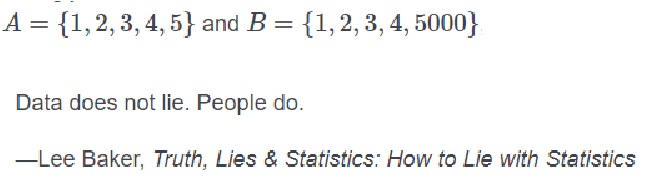
\includegraphics[scale=0.8]{params.jpg}
\end{frame}

\begin{frame}{Primer concepts in statistics}
	\uniitem{Consideration of sufficiency
		\uniitem{def: $f(\boldsymbol{x} | \boldsymbol{\theta}) = g(T(\boldsymbol{X} | \boldsymbol{\theta})) h(\boldsymbol{x})$}
		\uniitem{design intention of \code{StratifiedKFold} in \code{scikit-learn}}
		\uniitem{interpretation of bootstrap (CS) in statistics (convergency)}}
\end{frame}

\begin{frame}{Proposals in managing data practice}
	\uniitem{Diagnosis on samples (assume $\boldsymbol{A} \subset \boldsymbol{B} \subset \boldsymbol{C}$)
		\uniitem{$s(\boldsymbol{A})$ diff from $s(\boldsymbol{B})$ => increase nums. | test variants,}
		\uniitem{$\boldsymbol{A} \subset \boldsymbol{B} \rightarrow f$ be ineffective from $\boldsymbol{B}$ to $\boldsymbol{C}$ => data aquisition;}}
	\uniitem{Applicability of algorithm
		\uniitem{evaluate applicability from frame to task-objective,}
		\uniitem{modification | design => parameterization;}}
	\uniitem{Further works
		\uniitem{cleaning, preprocessing, training, validation, etc.}}
\end{frame}

\begin{frame}{Determination of algorithm design}
	\uniitem{Case 4: statistics on nuclei of cancer cells
		\uniitem{objective: $\mathcal{N}(\boldsymbol{x}, \boldsymbol{\Sigma})$ dis of nuclei, statistical approahces}}
	\centering
	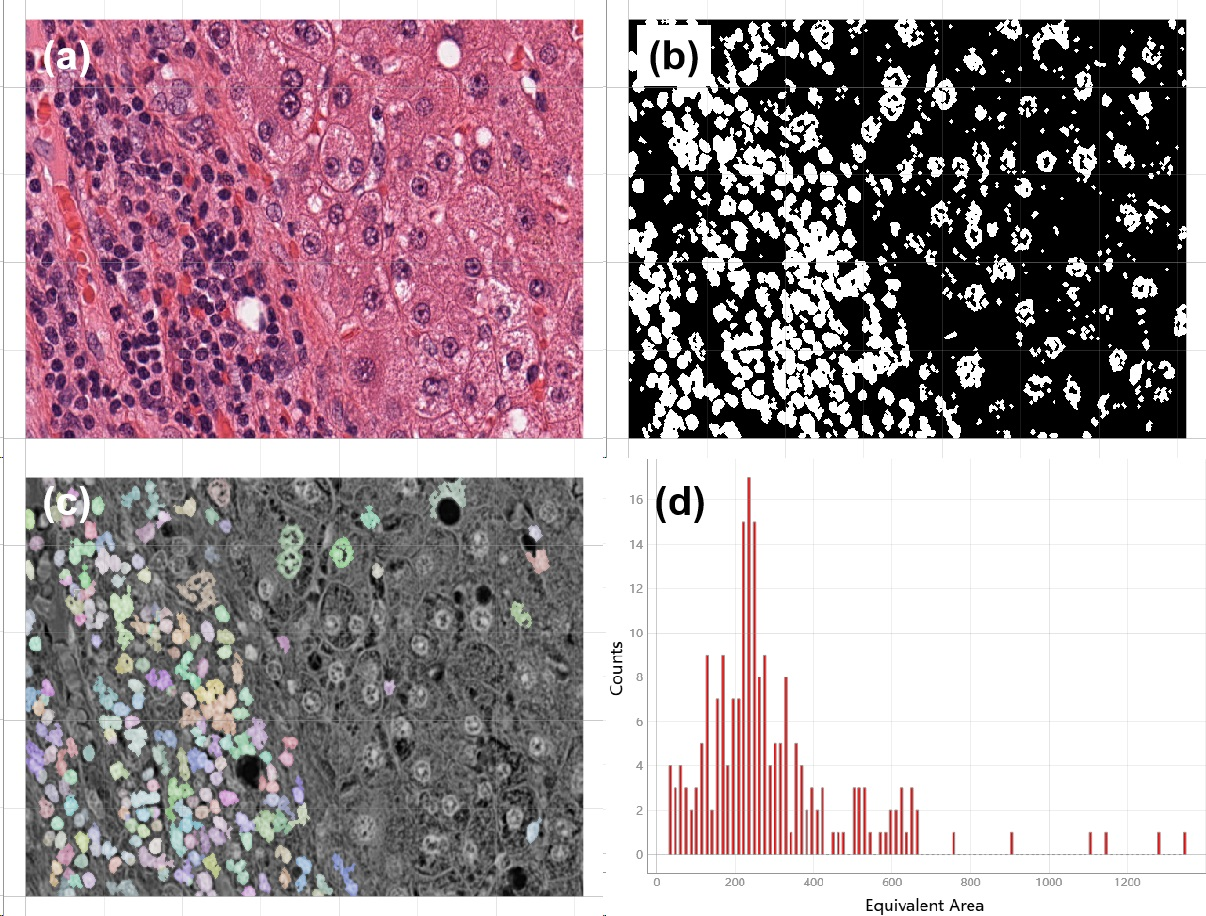
\includegraphics[scale=0.43]{patho.jpg}
\end{frame}

\begin{frame}{Determination of algorithm design}
	\uniitem{Case 4: statistics on nuclei of cancer cells
		\uniitem{diagnosis on dis => fat-tailed \& outliers}}
	\centering
	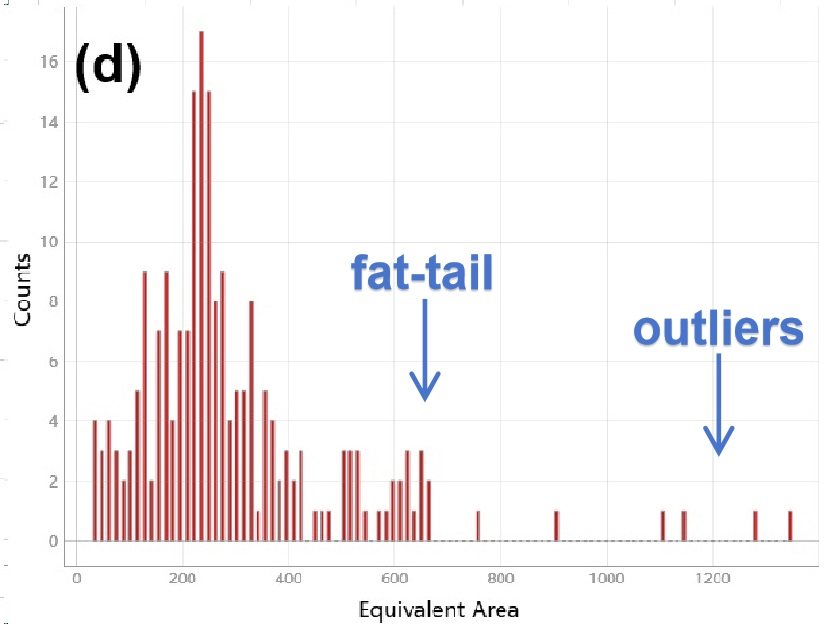
\includegraphics[scale=0.6]{pathlocal.jpg}
\end{frame}

\begin{frame}{Determination of algorithm design}
	\uniitem{Case 4: statistics on nuclei of cancer cells
		\uniitem{+MCMC aug => params converge in prob}}
	\centering
	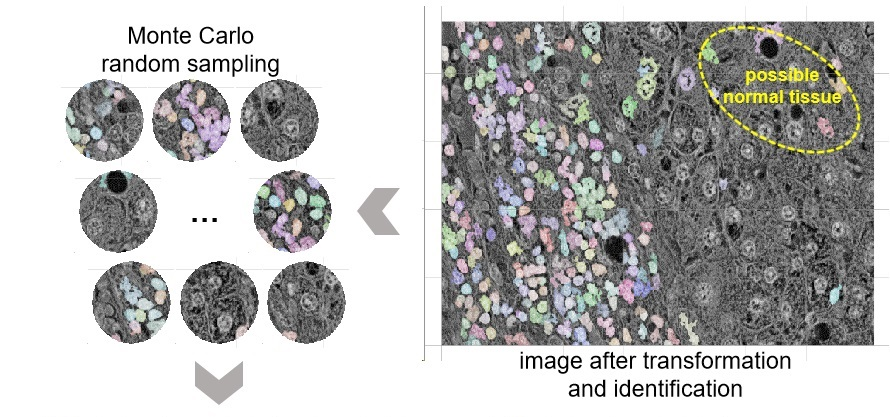
\includegraphics[scale=0.75]{mcmc1.jpg}
\end{frame}

\begin{frame}{Determination of algorithm design}
	\uniitem{Case 4: statistics on nuclei of cancer cells
		\uniitem{+MCMC aug => params converge in prob}}
	\centering
	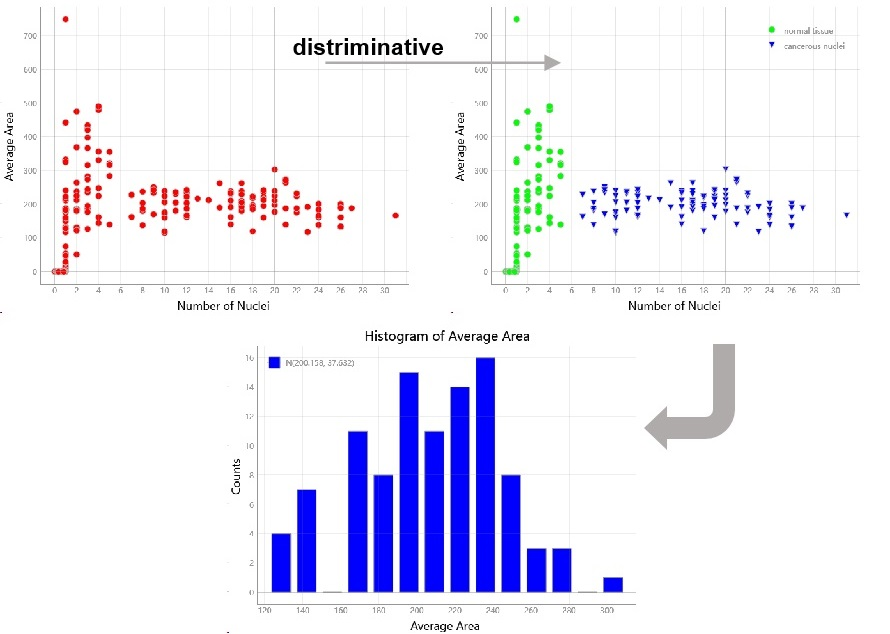
\includegraphics[scale=0.6]{mcmc2.jpg}
\end{frame}

\section{Anomaly recognition}

\subsection{Introduction: integration of scientific computation}

\begin{frame}{Comb. \& App. of multi sc meta implementations}
	\uniitem{Dis-related methods (e.g. T2, Naive Bayes)
		\uniitem{methematical statistics, hypothesis tests}
		\uniitem{linear algebra (supporting multivariate)}
		\uniitem{Bayes statistics and computation}}
	\uniitem{Data-related methods (e.g. neighbors)
		\uniitem{data structure (CS), \code{KDTree} for query}
		\uniitem{optimizations, for numeric solution}
		\uniitem{signal decomposition}
		\uniitem{linear algebra as well}}
	\uniitem{Other methods\dots}
\end{frame}

\begin{frame}{Comb. \& App. of multi sc meta implementations}
	\uniitem{Security:
		\uniitem{risky transaction, anti-fraud, \dots}}
	\uniitem{Quality ensurance:
		\uniitem{quality testing, mechanical fault monitoring, \dots}}
	\uniitem{Networks:
		\uniitem{spam recog., attack monitoring, \dots}}
	\uniitem{Medical:
		\uniitem{\asred{\textbf{less reported}}}}
\end{frame}

\subsection{Comprehension: concept and applicable scope}

\begin{frame}{Essentials: conventional hypothesis testing}
	\uniitem{One-side modeling: stats on one-class $\rightarrow$ normal/anomaly}
	\centering
	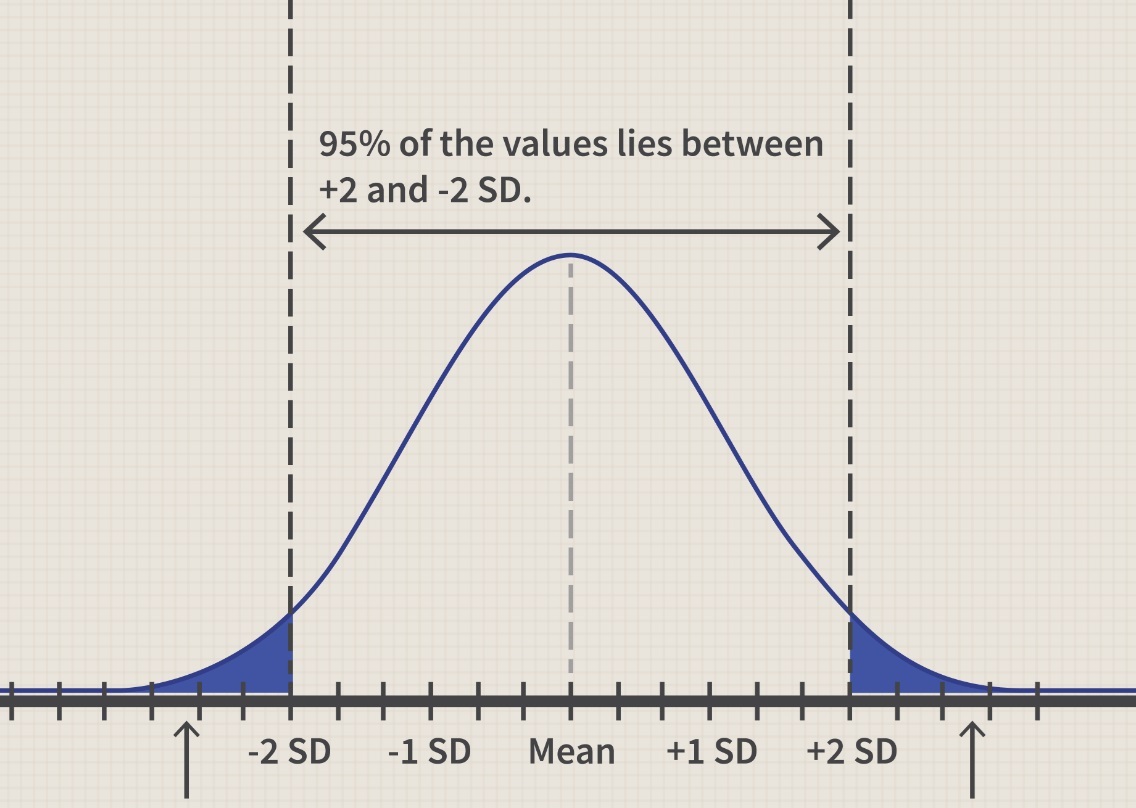
\includegraphics[scale=0.45]{hypotest.jpg}\\
	accept/rejection regions\footnote[frame]{\ftref{https://www.investopedia.com/articles/active-trading/092214/hypothesis-testing-finance-concept-examples.asp}{Hypothesis testing concepts and examples}}
\end{frame}

\begin{frame}{Essentials: concept and applicable scope}
	\uniitem{Anomaly detection\footnote[frame]{\ftref{https://informatics.readthedocs.io/en/latest/supplement/supp\_b2.html\#id1}{Anomaly and change}}:
		\uniitem{stats on one-class $\rightarrow$ accept/rejection $\rightarrow$ routine/anomaly-like}}
	\centering
	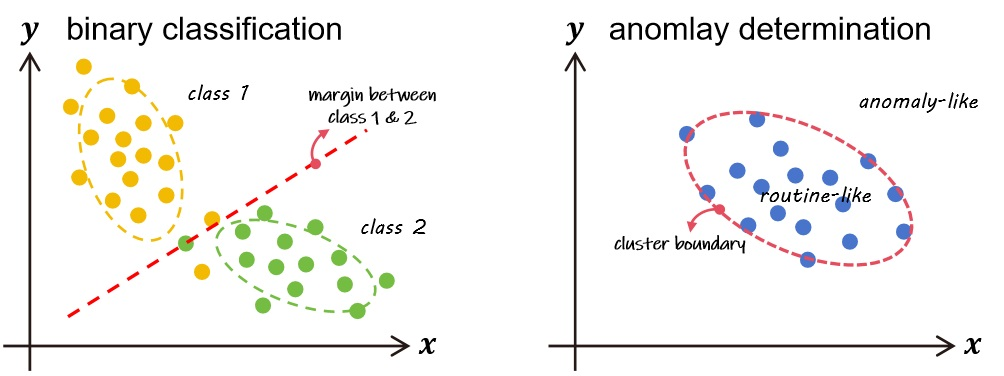
\includegraphics[scale=0.65]{anomaly.jpg}
\end{frame}

\begin{frame}{Essentials: concept and applicable scope}
	\emph{Why not binary classification?}\\
	\begin{minipage}[t]{0.5\textwidth}
		\uniitem{\textbf{binary classification}\\
			\begin{enumerate}
				\item narrow vs. narrow
				\item large data required
				\item low generalization
			\end{enumerate}}
    \end{minipage}%
    \hfill
    \begin{minipage}[t]{0.45\textwidth}
    	\uniitem{\textbf{anomaly detection}\\
			\begin{enumerate}
				\item narrow vs. generic
				\item low data required
				\item high generalization
			\end{enumerate}}
    \end{minipage}
    \vfill
    \asred{\textbf{Source: limited capability for unknown pattern}}
\end{frame}

\subsection{Applications: principles and implementations}

\begin{frame}{Hotelling T2:\footnote[frame]{\ftref{https://informatics.readthedocs.io/en/latest/supplement/supp\_b2.html\#id3}{Hotelling T-squared}} multivariate student-T}
	\uniitem{\textbf{Hypothesis:}
		\uniitem{null: case is derived from the identical population,}
		\uniitem{alternative: case is not derived from the identical population;}}
	\uniitem{\textbf{T2 statistic:}\\
		\qquad $T^2 = \frac{N-M}{(N+1)M} (\boldsymbol{x}^\prime - \hat{\boldsymbol{\mu}})^\top \hat{\boldsymbol{\Sigma}}^{-1} (\boldsymbol{x}^\prime - \hat{\boldsymbol{\mu}}) \sim F(M, N-M)$}
	\uniitem{\textbf{Criterion:}\\
		\qquad $(\boldsymbol{x}^\prime - \hat{\boldsymbol{\mu}})^\top \hat{\boldsymbol{\Sigma}}^{-1} (\boldsymbol{x}^\prime - \hat{\boldsymbol{\mu}}) \sim \chi^2 (x | M, 1)$}
	\vfill
	calculation on basis of $\chi^2 (x | M, 1)$
\end{frame}

\begin{frame}{Large margin nearest neigbors (LMNN)}
	\uniitem{Essential concept: \emph{homeomorphism\footnote[frame]{\ftref{https://en.wikipedia.org/wiki/Homeomorphism\#:\~:text=In\%20mathematics\%20and\%20more\%20specifically,has\%20a\%20continuous\%20inverse\%20function.}{Topological isomorphism}}}}
	\centering
	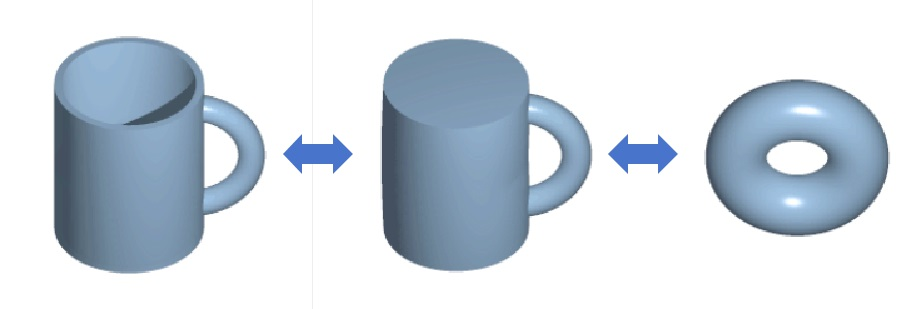
\includegraphics[scale=0.8]{homeomorphism.jpg}
\end{frame}

\begin{frame}{LMNN: role of Riemannian space}
	\begin{minipage}[t]{0.5\textwidth}
		Euclidean (global ops)\\
		$\boldsymbol{x}^\prime = f(\boldsymbol{x}) = \boldsymbol{Ax}$
		\centering
		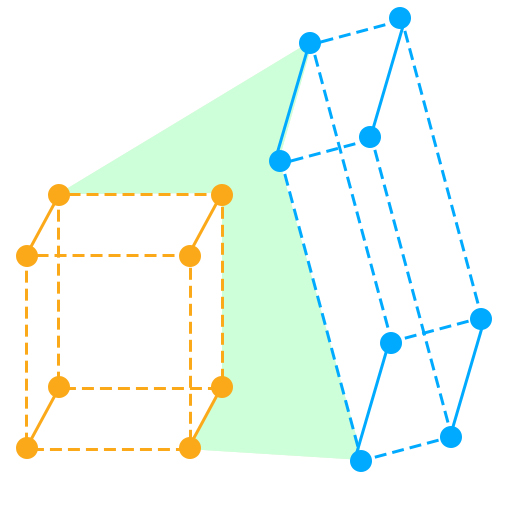
\includegraphics[scale=0.85]{matrix-trans.jpg}
    \end{minipage}%
    \hfill
    \begin{minipage}[t]{0.45\textwidth}
    	Riemannian (local ops)\\
    	$\boldsymbol{x}^\prime = f(\boldsymbol{x}) = \boldsymbol{Bx}$
    	\centering
    	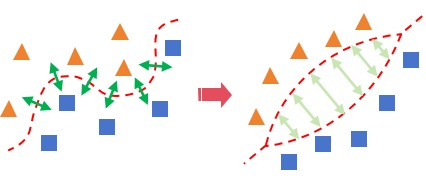
\includegraphics[scale=0.85]{riemannian-trans.jpg}
    	\begin{itemize}
    		\item The determination of $\boldsymbol{B}$?
    	\end{itemize}
    \end{minipage}
\end{frame}

\begin{frame}{LMNN: problem description\footnote[frame]{\ftref{https://informatics.readthedocs.io/en/latest/supplement/supp\_b2.html\#id4}{Empirical distribution and neighbors}}}
	\uniitem{\textbf{Optimization objective}:\\
		\[\Psi (\boldsymbol{R}) = \frac{1}{N} \sum_{c=1}^s \sum_{n=1}^N \left[ w_c \cdot \psi_1^{(n)} (\boldsymbol{R}) + \sum_{m \in \{c\}^C} w_m \cdot \psi_2^{(n)} (\boldsymbol{R}) \right]\]}
	\uniitem{\textbf{Constraints}:\\
		\[ \mathrm{s.t.} \> \boldsymbol{R} \succeq 0 \]}
	\uniitem{\textbf{Supports}:\\
		\code{linalg}, matrix decomp., data structure, \dots}
\end{frame}

\begin{frame}{LMNN: optimization \& Riemannian space}
	\[ \mathop{\arg\min}_{\boldsymbol{R}} \Psi (\boldsymbol{R}) \rightarrow \boldsymbol{R}^* \]
	\uniitem{matrix decomposition: LDLt\\
		\[ \boldsymbol{R}^* =  \boldsymbol{L_m \Lambda_m L_m}^\top =  \boldsymbol{L \Lambda \Lambda}^\top \boldsymbol{ L}^\top\]
		\[ \therefore \boldsymbol{L}^\prime = \boldsymbol{L \Lambda} \]}
	\uniitem{Cartesian to Riemannian space:\\
		\[ f(\boldsymbol{x}) = \boldsymbol{L}^\prime \boldsymbol{x} \]}
\end{frame}

\begin{frame}{Anomaly detection: decoupling the AI algorithms}
	\uniitem{As for general case:
		\uniitem{normal/anomaly determination;}}
	\uniitem{As for anomaly cases:
		\uniitem{expertise model for subtypes (most researchers mainly do);}}
	\uniitem{As for interested subtypes:
		\uniitem{further investigation for principles/mechanisms;}}
	\uniitem{Well recoginized $\rightarrow$ full utilization:
		\uniitem{model to export (suggested) decision, etc.}}
\end{frame}

\section{Summary}

\begin{frame}{AI algorithm in practice}
	\uniitem{The relations between AI algorithm and scientific computation}
	\begin{minipage}[t]{0.5\textwidth}
		\vspace{0pt}
		\centering
		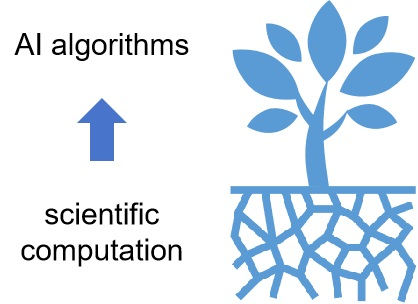
\includegraphics[scale=0.85]{tree.jpg}
    \end{minipage}%
    \hfill
    \begin{minipage}[t]{0.45\textwidth}
        \vspace{0pt}
        \begin{enumerate}
        	\item \textbf{SC} $\rightarrow$ AI $\rightarrow$ App.\\
        		\uniitem{technical methods set}
        		\uniitem{rational combination}
			\item objective $\rightarrow$ AI frame\\
				\uniitem{high generalization}
				\uniitem{expertise for problem}
				\uniitem{interpretability}
        \end{enumerate}
    \end{minipage}
\end{frame}

\begin{frame}{Mottos: }
	\uniitem{There is neither elixir for all diseases in this world, nor generic solution for all questions.\footnote[frame]{\ftref{https://informatics.readthedocs.io/en/latest/supplement/supp\_a1.html\#id4}{Pattern in high dimensional data}}}
	\uniitem{Invocation without coprehension is just like tree without root, stream without source.}
	\uniitem{Scientific computation and rationality: the motivation and reason of finding the information underlying the data.}
\end{frame}

\end{document}